\documentclass[11pt, a4paper]{article}
\usepackage[utf8]{inputenc}
\usepackage[left=2cm, right=2cm, top=2.5cm, bottom=2.0cm]{geometry}
\usepackage{amsmath, amssymb, amsthm}
\usepackage[english]{babel}
\usepackage{graphicx}
\usepackage[font={small,it}]{caption}
\graphicspath{ {figures/} }
\usepackage{url}
\usepackage{appendix}
\usepackage{float}
\usepackage[bottom]{footmisc}
\usepackage{titling}
\setlength{\droptitle}{-10em}  

\title{ \huge Artificial neural networks \\ 
  { \large Assignment 1: Supervised learning and generalization }}
\author{
        Lood, Cedric \\
        \small Master of Bioinformatics
}

\begin{document}
\maketitle
%\tableofcontents

\section{Context}

Artificial neural networks that have at least 1 hidden layer have the
property of being universal
approximator\cite{hornik1989multilayer,leshno1993multilayer}. Hence,
any non-linear function can be realized using classical feedforward
multilayers networks. Here, I explore different training algorigthm
and compare their yields in terms of performance, training time, and
generalization. For the sake of simplification, I used the underlying,
known function $f(x)=e(-x^2)sin(10x)$ to generate the dataset for
batch supervised learning. The architecture of the neural network
consists of 10 hidden units with sigmoid transfer function, 1 input,
and 1 output (linear).

\section{Noise-free learning}

The function $f(x)$ was learned using noiseless datapoints over the
range $[-\pi;\pi]$ by interval of $\delta x = 0.1$. The training
algorithm selected are the ones reviewed during the lecture. Their
relative performances can be appreciated by looking at the figure
\ref{fig:trainnl}. On the left-hand side, the approximation of the
different learning schemes after 100 epochs. On the right-hand side,
the training error as it evolve during training.:

\begin{figure}[H]
  % \centering
  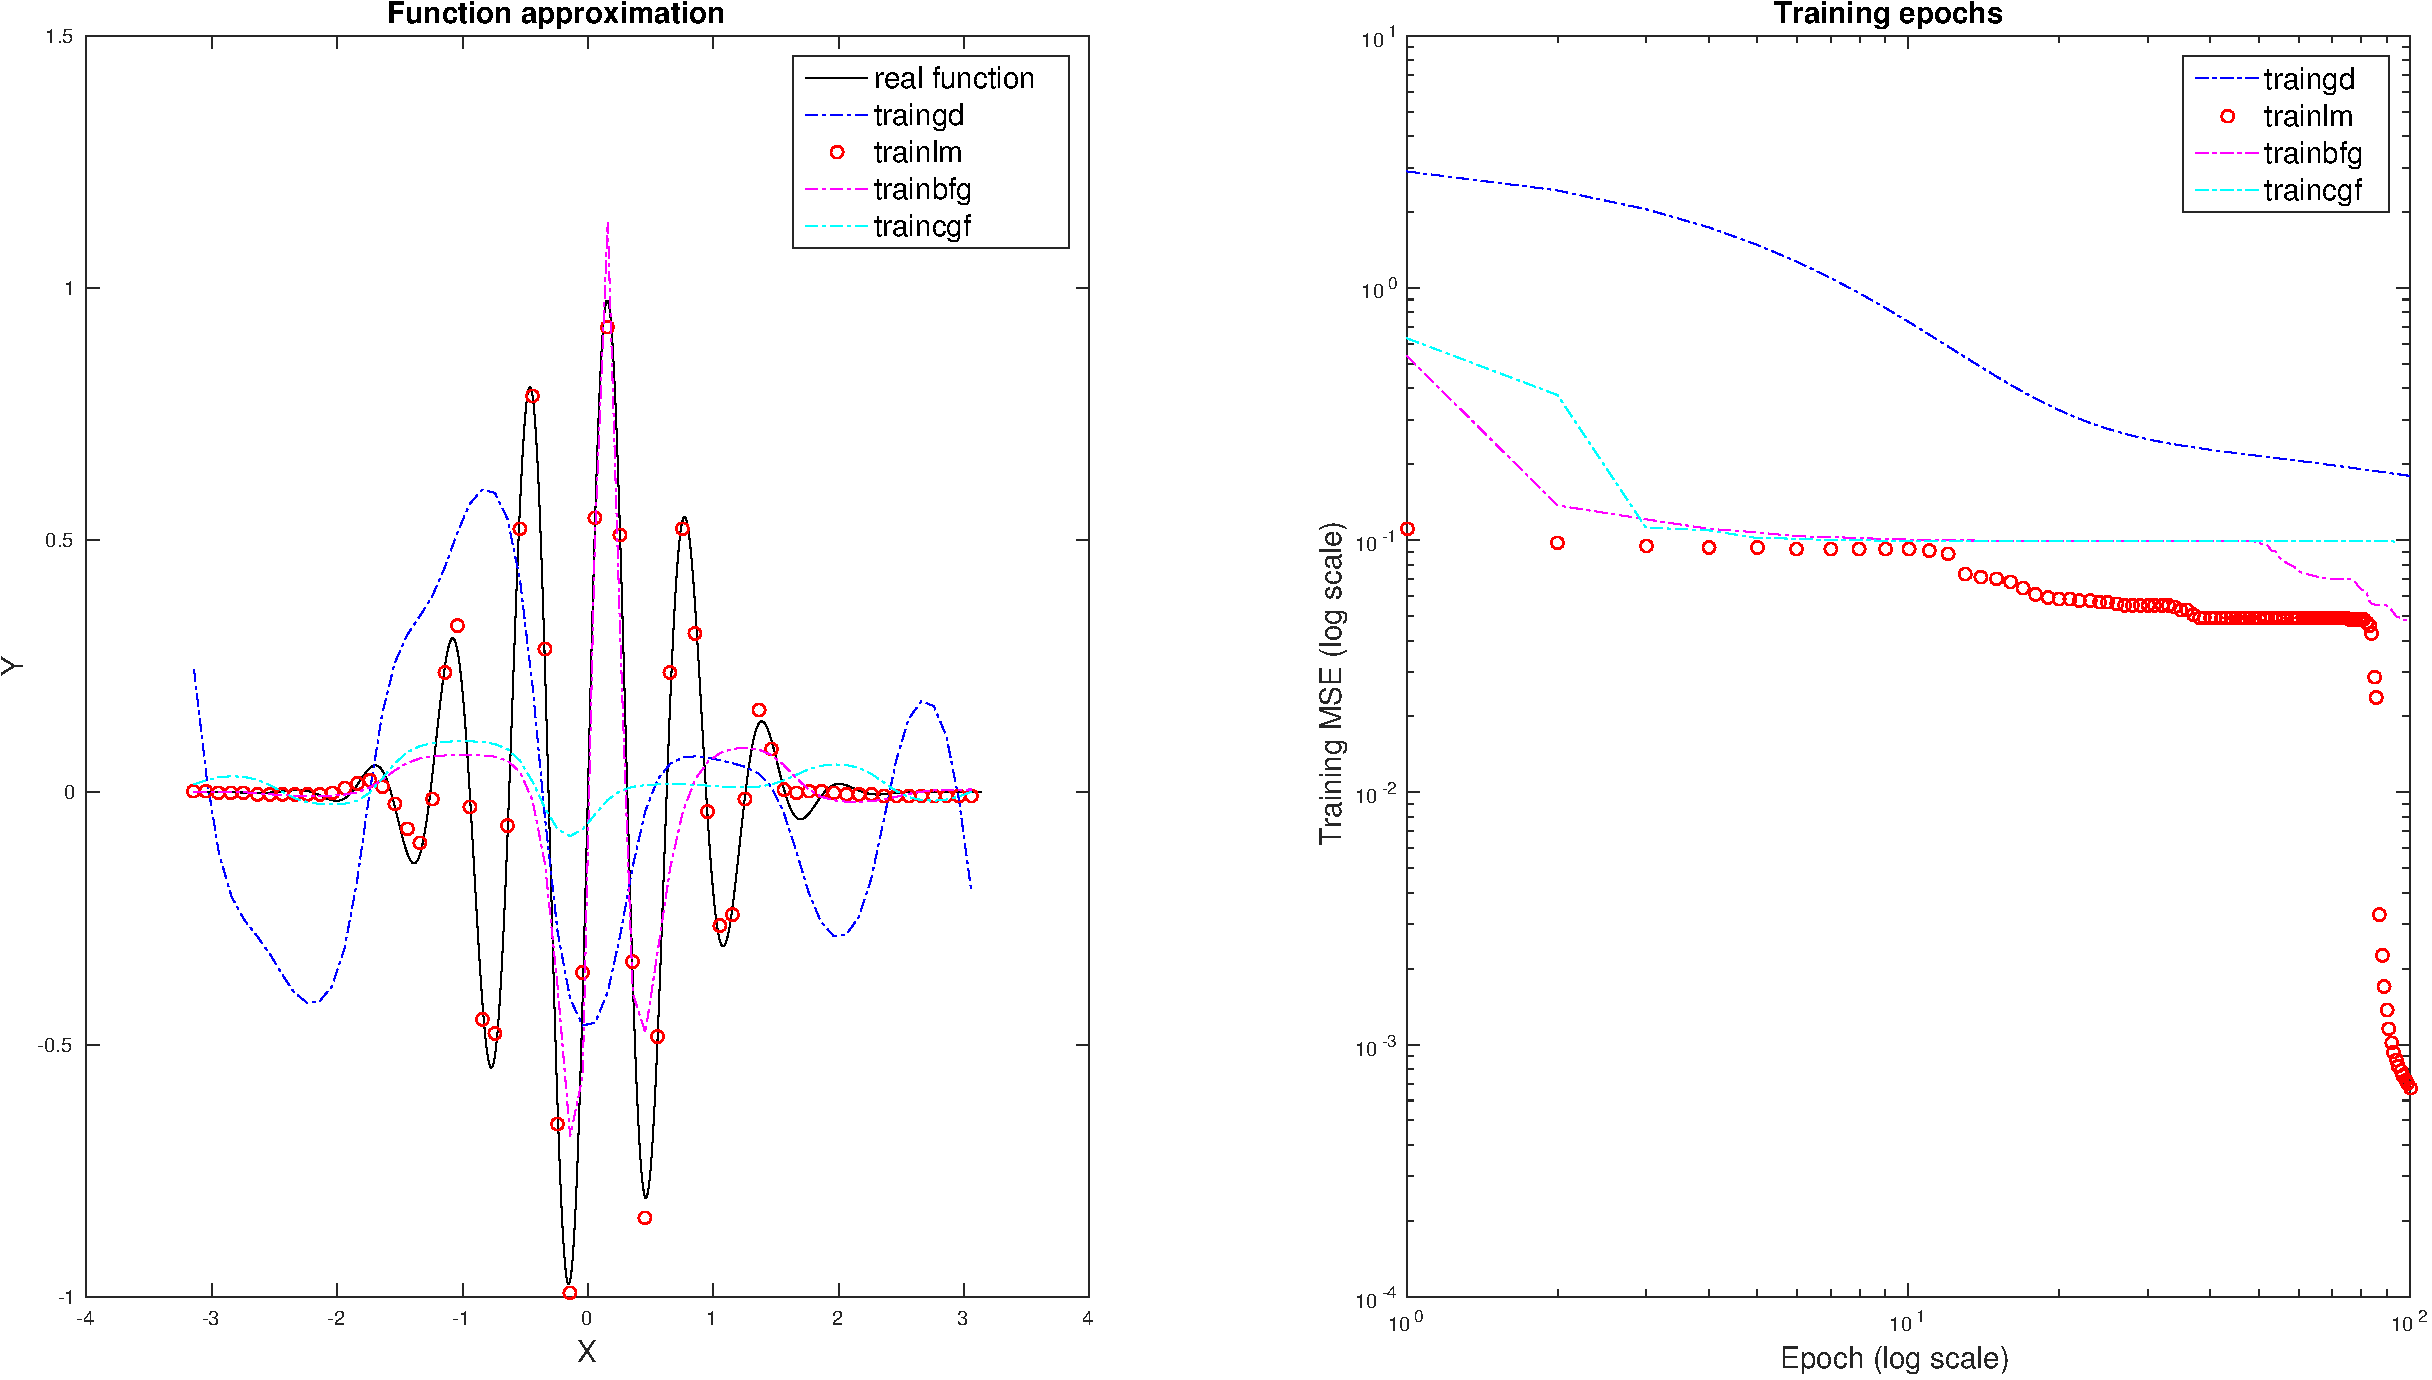
\includegraphics[scale=.43]{training_performance.pdf}
  \caption{Training performance}
  \label{fig:trainnl}
\end{figure}

\begin{description}
\item [traingd] is the gradient descent algorithm. Its performance
  were rather terrible in terms of function approximation. The
  implementation details are simple, but it suffers from slow
  convergence.
\item [trainlm] was the best performer overall with the different
  functions I tried to approximate. The algorithm ressembles the
  Newton method but has an extra-term that enables solving otherwise
  ill-conditioned problems.
\item [trainbfg] is a quasi-Newton method. This algorithm avoids the
  computation of the Hessian matrix, and works instead with an
  approximation, sparing CPU cycles.
\item [traincgf] is a conjugate gradient approach, which can be really
  useful when dealing with networks that have a lot of hidden neurons
  and/or interconnections. This algorithm avoids storing the Hessian
  matrix, sparing the RAM needed otherwise to store potentially huge
  matrices.
\end{description}

\section{Learning in noisy setting}

For this section, I worked with a slightly easier function
$f(x)=x^3-11x+2$. To simulate the presence of noise in the dataset, I
chose to add a normally distributed $\epsilon$ to $f(x)$, for example:
$f_{noisy}=f(x)+N(0,1)$.

See graphic \ref{fig:trainnoise} where the noisy dataset was used for
training. Typical overfitting can be seen when raising the value of
the \emph{epochs}, represented in the graph by the red curve, which
upon closer inspection seems to be following the noise rather than
fitting the underlying function. Strategies to decide when to stop
training can be implemented, such as validation set, cross validation,
and bootstrapping.

\begin{figure}[H]
  % \centering
  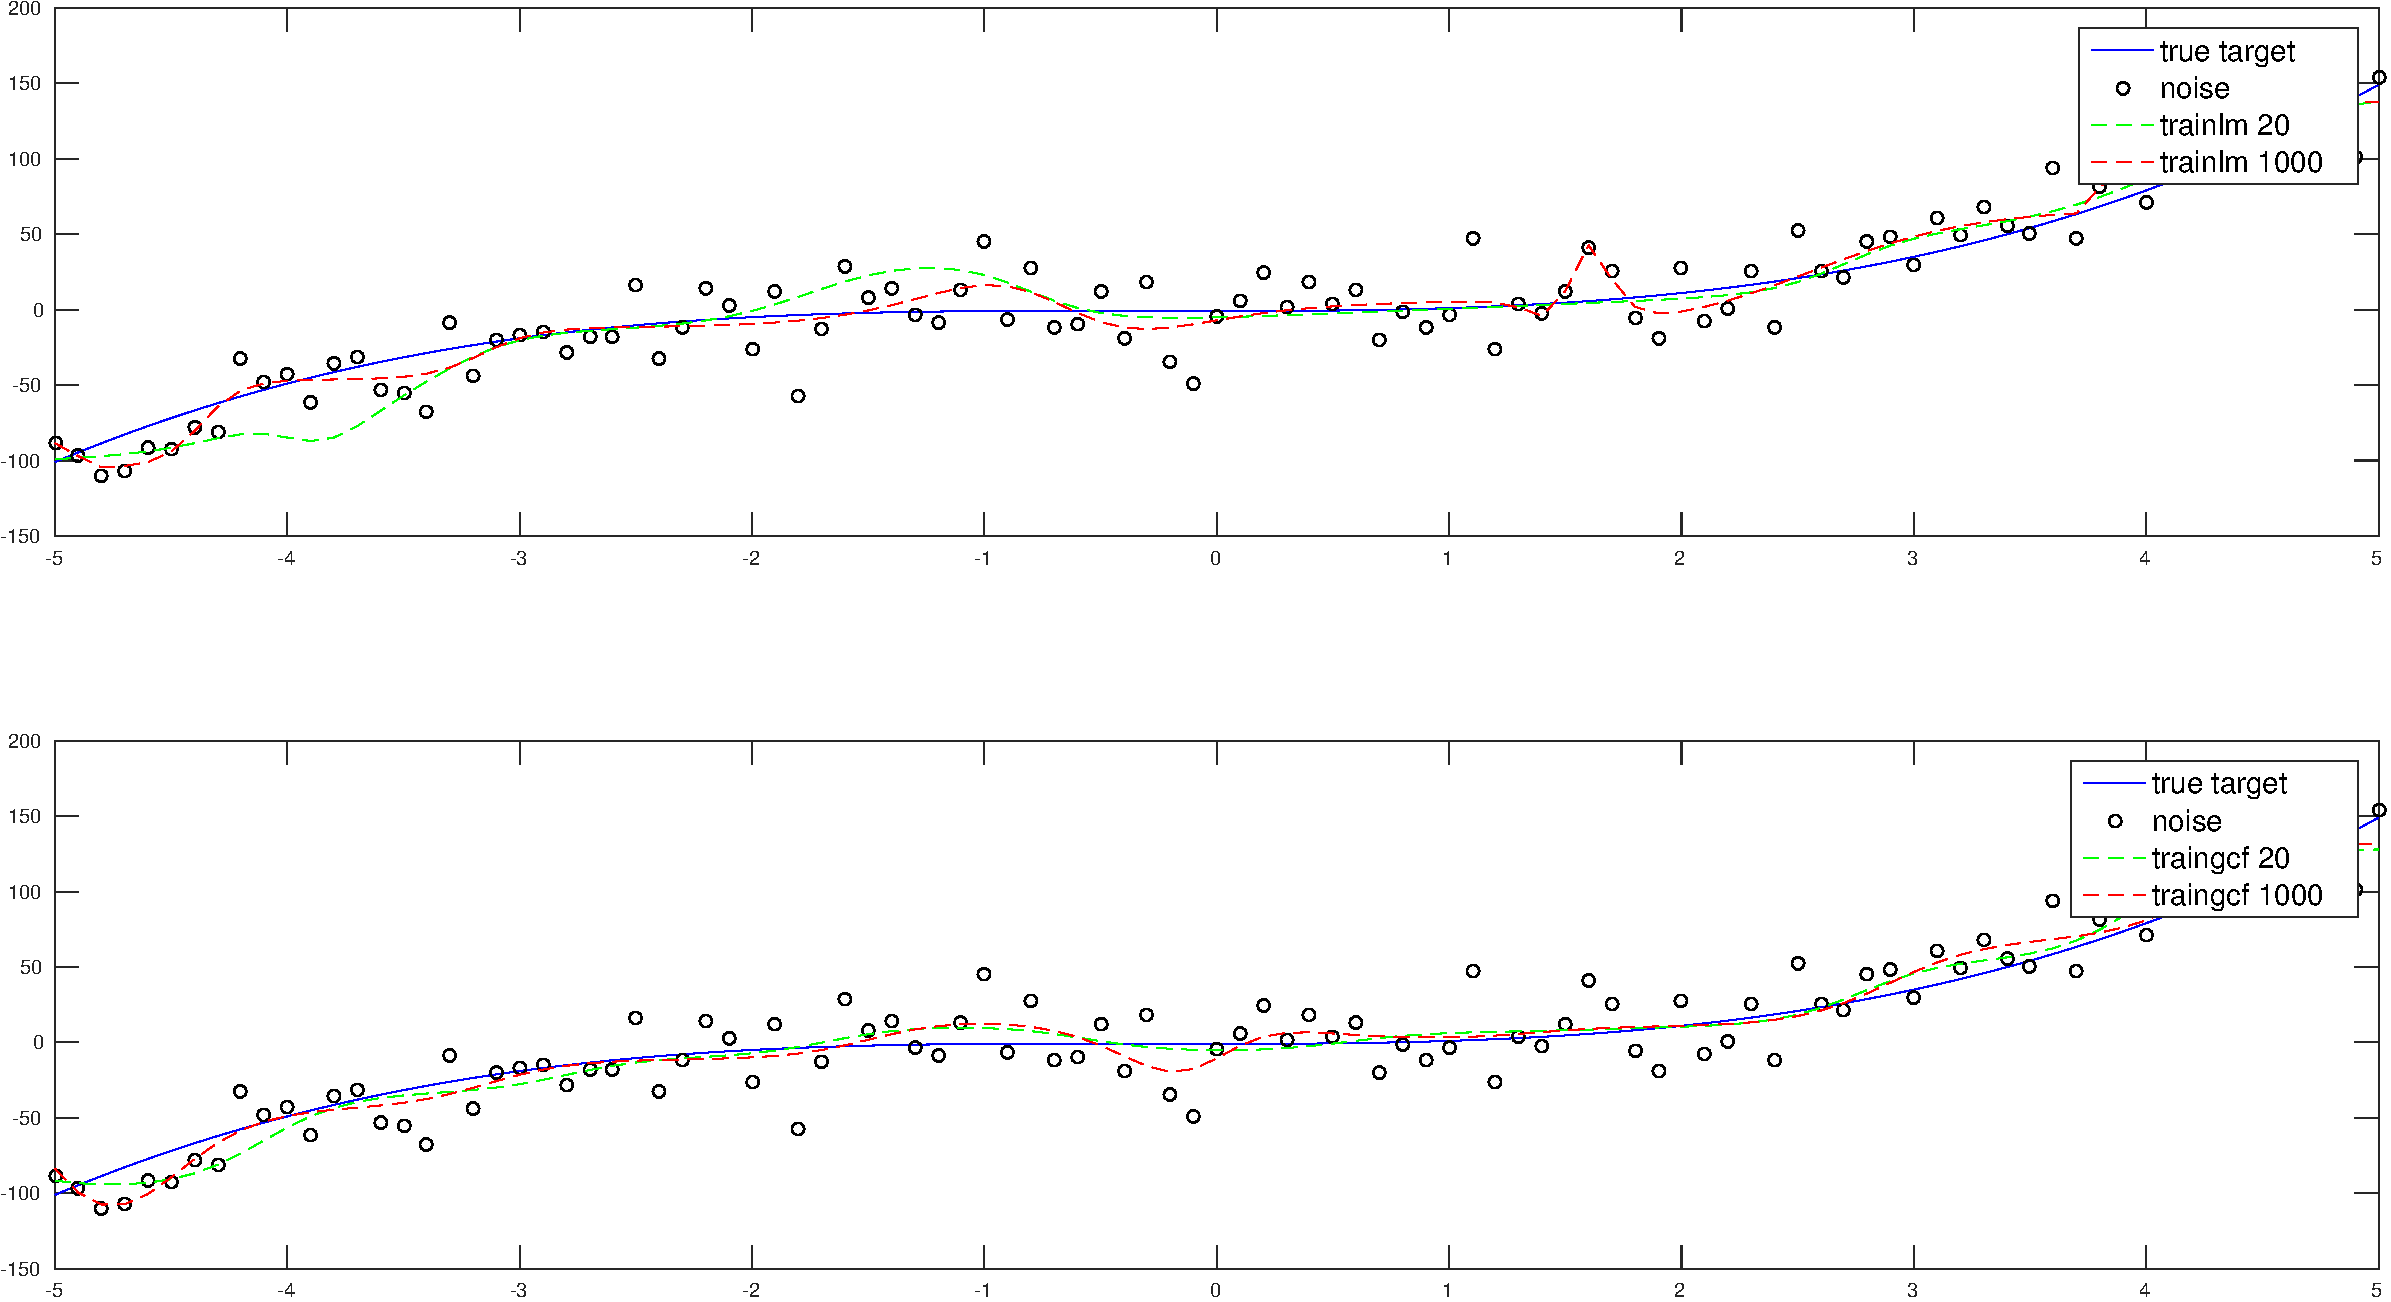
\includegraphics[scale=.43]{trainnoise.pdf}
  \caption{Example of overfitting in noisy dataset}  
  \label{fig:trainnoise}
\end{figure}

{\footnotesize
\bibliographystyle{ieeetr} 
\bibliography{bib-db}}

\end{document}
